\documentclass[conference]{IEEEtran}

\usepackage{amsmath,amssymb,amsfonts}
\usepackage{booktabs}
\usepackage{multirow}
\usepackage{graphicx}
\usepackage{array}
\usepackage{url}
\usepackage{cite}
\usepackage{xcolor}
\usepackage{tikz}
\usepackage{algorithm}
\usepackage{algpseudocode}
\usepackage{enumitem}
\usepackage{microtype}
\usetikzlibrary{arrows.meta,positioning,fit}

\newcommand{\method}{\textsc{CropState}}
\newcommand{\softmax}{\operatorname{softmax}}
\newcommand{\argmaxop}{\operatorname*{arg\,max}}

\title{\method: Image-Driven Confidence-Aware Growth-Stage-Gated Retrieval for Rice Decision Support}

\author{\IEEEauthorblockN{L\^e B\hspace{0.05em}a\hspace{0.05em}o Nhi}
\IEEEauthorblockA{FPT University\\
Da Nang, Vietnam\\
lebaonhi0805@gmail.com}}

\begin{document}
\maketitle

\begin{abstract}
Agricultural management actions depend strongly on crop development, yet many decision-support systems retrieve evidence using only lexical or semantic similarity. A passage may therefore be topically relevant while being inappropriate for the current rice growth stage. This paper proposes \method, an image-driven, confidence-aware growth-stage-gated retrieval framework for rice decision support. A vision model first processes a field image and produces a probability distribution over six BBCH-derived rice macro-stages. Rather than converting this distribution immediately into a single hard label, \method preserves uncertainty, optionally fuses it with a temporal prior, and adaptively controls the contribution of stage compatibility during retrieval. The downstream component uses fixed care topics rather than free-form chatbot questions, combines BM25 and dense retrieval using normalized Reciprocal Rank Fusion, and returns structured stage-specific evidence. The study addresses two research questions: how accurately rice growth stages can be recognized from field images, and whether confidence-aware soft gating is more robust than top-1 hard filtering when image-based stage predictions are uncertain or incorrect. The protocol includes image-classification baselines, calibration analysis, oracle-stage retrieval, end-to-end image-based retrieval, the Stage-Inappropriate Retrieval Rate, robustness degradation, ablation studies, and paired statistical analysis. A pilot held-out vision experiment comparing three trained models (a from-scratch shallow CNN, fine-tuned ResNet-18, and fine-tuned EfficientNet-B0) plus a multi-seed check has been run and is reported; it gives a preliminary, favorable signal on rice growth-stage recognizability, but a paired, Holm-corrected statistical comparison finds no significant difference among the three trained models at this sample size, and the pilot split still lacks the real field/season grouping the protocol requires. Retrieval evaluation has not been run, and no claim on the comparative robustness of confidence-aware soft gating versus hard filtering is made until it is.
\end{abstract}

\begin{IEEEkeywords}
rice growth stage, computer vision, BBCH, image classification, retrieval-augmented generation, uncertainty-aware retrieval, agricultural decision support
\end{IEEEkeywords}

\section{Introduction}
Agricultural recommendations are conditional on crop development. Water management, nutrient application, disease risk, weed control, and harvest preparation can change substantially between establishment, tillering, reproductive development, grain filling, and ripening. A retrieval system that ignores growth stage may return evidence that is semantically related to the topic but mistimed in agronomic application.

A practical system must also determine the current stage without requiring a user to formulate a technical question. Field images provide a natural input because phenological development is partially observable from plant morphology. However, image-based stage recognition is uncertain, especially near stage boundaries, under poor lighting, or when images from different fields and seasons vary in background and scale. Converting an uncertain visual prediction into a single stage label and applying a hard metadata filter may amplify classification errors by removing all evidence associated with the true stage.

This paper proposes \method, an image-driven pipeline that connects rice growth-stage recognition to stage-aware retrieval. The vision model outputs a distribution rather than only a top-1 class. This distribution becomes a stage belief that controls how strongly the retriever favors stage-compatible evidence. When the visual prediction is concentrated and calibrated, stage compatibility receives more weight. When it is diffuse or conflicts with a temporal prior, the system relaxes stage conditioning to preserve recall.

The system is not designed as a free-form chatbot. After an image is uploaded, it automatically retrieves evidence for a fixed set of care topics such as water, nutrients, disease risk, pest risk, and weed management. Outputs are structured as detected stage, confidence, stage-specific recommendations, and supporting sources.

The intended contributions are:
\begin{enumerate}[leftmargin=*,nosep]
    \item an image-driven pipeline that links six-class rice growth-stage recognition to structured agricultural retrieval;
    \item a confidence-aware soft-gating method that uses the full visual probability distribution instead of only the top-1 stage;
    \item an end-to-end evaluation protocol that measures how vision uncertainty and classification errors propagate to retrieval quality and stage-inappropriate evidence.
\end{enumerate}

\begin{figure}[!t]
\centering
\resizebox{\columnwidth}{!}{%
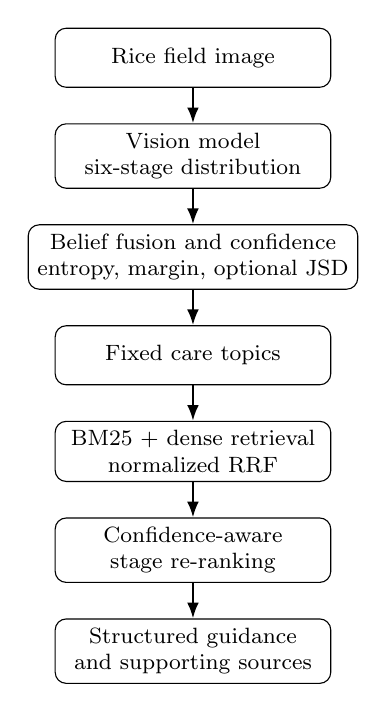
\begin{tikzpicture}[
node distance=4.5mm,
box/.style={draw,rounded corners,align=center,minimum width=35mm,minimum height=7.5mm,font=\footnotesize},
arr/.style={-{Latex[length=2mm]},thick}
]
\node[box] (img) {Rice field image};
\node[box,below=of img] (vision) {Vision model\\six-stage distribution};
\node[box,below=of vision] (belief) {Belief fusion and confidence\\entropy, margin, optional JSD};
\node[box,below=of belief] (topics) {Fixed care topics};
\node[box,below=of topics] (retrieve) {BM25 + dense retrieval\\normalized RRF};
\node[box,below=of retrieve] (rerank) {Confidence-aware\\stage re-ranking};
\node[box,below=of rerank] (output) {Structured guidance\\and supporting sources};
\draw[arr] (img)--(vision);
\draw[arr] (vision)--(belief);
\draw[arr] (belief)--(topics);
\draw[arr] (topics)--(retrieve);
\draw[arr] (retrieve)--(rerank);
\draw[arr] (rerank)--(output);
\end{tikzpicture}}
\caption{Image-driven \method pipeline without free-form chatbot interaction.}
\label{fig:pipeline}
\end{figure}

\section{Related Work}
\subsection{Retrieval-Augmented Generation and Hybrid Retrieval}
Retrieval-Augmented Generation grounds model outputs in external evidence \cite{lewis2020rag}. Sparse retrieval such as BM25 captures lexical correspondence \cite{robertson2009bm25}, while dense retrieval captures semantic similarity \cite{karpukhin2020dpr}. Reciprocal Rank Fusion (RRF) combines ranked lists without directly comparing heterogeneous raw scores \cite{cormack2009rrf}. \method uses BM25 and dense retrieval for candidate generation, then applies confidence-aware stage re-ranking.

\subsection{Agricultural Context-Aware Retrieval}
Crop GraphRAG organizes crop-protection knowledge around crop--pest--disease--symptom--control relations and performs graph-based evidence aggregation. Its primary contribution is relational knowledge structure rather than uncertainty in a visually estimated crop state. AgriRegion conditions retrieval on geographic metadata to reduce recommendations that are valid in one region but inappropriate in another. In contrast, \method conditions retrieval on an ordered phenological state inferred from images and explicitly evaluates robustness when that state estimate is wrong. Table~\ref{tab:positioning} summarizes the distinction.

\begin{table*}[t]
\caption{Positioning relative to closely related retrieval directions.}
\label{tab:positioning}
\centering
\footnotesize
\begin{tabular}{p{0.15\textwidth}p{0.20\textwidth}p{0.23\textwidth}p{0.32\textwidth}}
\toprule
Direction & Primary context & Main retrieval mechanism & Difference from \method \\
\midrule
Standard RAG & Query content & Sparse/dense passage retrieval & Does not model phenological applicability. \\
Crop GraphRAG & Crop--pest--symptom--control relations & Local/global graph retrieval & Focuses on relational structure, not image-derived stage belief or stage-error robustness. \\
AgriRegion & Geographic region and local sources & Region-prioritized re-ranking & Uses geographic context rather than ordered visual phenology. \\
\method & Image-derived rice stage belief & Confidence-adaptive soft re-ranking & Evaluates propagation of visual uncertainty into stage-specific retrieval. \\
\bottomrule
\end{tabular}
\end{table*}

\subsection{Rice Growth-Stage Recognition}
The BBCH scale provides standardized phenological codes for crop development \cite{meier2001bbch,lancashire1991uniform}. Prior work has shown that machine-learning methods can recognize rice growth stages from imagery \cite{tan2022rice}. Modern image classifiers commonly use pretrained convolutional or transformer backbones, and calibration methods such as temperature scaling can improve the relationship between predicted confidence and empirical correctness \cite{he2016resnet,tan2019efficientnet,guo2017calibration}.

The present work does not claim a new vision architecture. The scientific focus is the interface between visual stage uncertainty and retrieval. The vision model is an upstream estimator whose full output distribution is retained for downstream decision support.

\section{Problem Formulation}
\subsection{Growth-Stage Space}
Let $\Phi=\langle\phi_1,\ldots,\phi_m\rangle$ denote an ordered set of rice growth stages. The initial study uses the six macro-stages in Table~\ref{tab:stages}. These groups are an experimental abstraction of BBCH codes rather than a new phenological standard. The primary task is whole-image classification. Object detection is outside the main evaluation and may only be used as an auxiliary localization method.

\begin{table}[t]
\caption{Rice macro-stages used in the planned benchmark.}
\label{tab:stages}
\centering
\footnotesize
\begin{tabular}{p{0.46\columnwidth}p{0.18\columnwidth}p{0.22\columnwidth}}
\toprule
Group & BBCH & Label \\
\midrule
Germination and leaf development & 00--19 & Establishment \\
Tillering & 20--29 & Tillering \\
Stem elongation and booting & 30--49 & Stem/booting \\
Heading and flowering & 50--69 & Reproductive \\
Grain development & 70--79 & Grain filling \\
Ripening & 80--89 & Ripening \\
\bottomrule
\end{tabular}
\end{table}

\subsection{Image-Based Stage Belief}
For rice image $I_t$, a vision model with parameters $\theta$ produces logits $\mathbf{o}_t=f_{\theta}(I_t)$. The visual stage distribution is
\begin{equation}
p_{\mathrm{vis},t}=\softmax(\mathbf{o}_t/T),
\end{equation}
where $T>0$ is a temperature parameter estimated on the validation set. The top-1 prediction is
\begin{equation}
\widehat{\phi}_t=\argmaxop_i p_{\mathrm{vis},t}(\phi_i),
\end{equation}
but \method retains the complete distribution instead of discarding non-maximal stages.

\subsection{Optional Temporal Prior and Fusion}
If sowing or transplanting time is available, a temporal vector $p_{\mathrm{time},t}$ can be constructed from agronomic development intervals. A transition matrix $A\in[0,1]^{m\times m}$ defines plausible progression from a previous belief $B_{t-1}$:
\begin{equation}
\widetilde{B}_t=A^{\top}B_{t-1}.
\end{equation}
Given prior weight $w_p$ and evidence weights $w_e$, log-linear fusion is
\begin{equation}
z_i=w_p\log(\widetilde{B}_t(\phi_i)+\epsilon)
+\sum_{e\in\mathcal{E}_t}w_e\log(p_e(\phi_i)+\epsilon),
\end{equation}
followed by
\begin{equation}
B_t(\phi_i)=\frac{\exp(z_i)}{\sum_j\exp(z_j)}.
\end{equation}
In the image-only configuration, $B_t=p_{\mathrm{vis},t}$. In the fused configuration, $\mathcal{E}_t$ contains visual and temporal evidence.

\subsection{Confidence and Source Agreement}
Belief concentration is measured using normalized entropy:
\begin{equation}
\Gamma_t=1-\frac{H(B_t)}{\log m},\qquad
H(B_t)=-\sum_i B_t(\phi_i)\log B_t(\phi_i).
\end{equation}
A complementary top-two margin is
\begin{equation}
M_t=B_t^{(1)}-B_t^{(2)},
\end{equation}
where $B_t^{(1)}$ and $B_t^{(2)}$ are the largest and second-largest belief values.

When both visual and temporal distributions are available, agreement is
\begin{equation}
G_t=1-\frac{\operatorname{JSD}(p_{\mathrm{vis},t},p_{\mathrm{time},t})}{\log 2}.
\end{equation}
The confidence proxy is defined as
\begin{equation}
\kappa_t=\eta_1\Gamma_t+\eta_2M_t+\eta_3G_t,
\end{equation}
where $\eta_1+\eta_2+\eta_3=1$. In the image-only configuration, $\eta_3=0$. This confidence is a routing signal, not proof that the predicted stage is correct.

\subsection{Documents and Stage Compatibility}
Let $\mathcal{D}$ be a collection of agricultural knowledge chunks. Each chunk $d$ includes source provenance, care topic, applicability metadata, and a compatibility vector
\begin{equation}
C(d,\phi_i)\in[0,1].
\end{equation}
A value of one denotes direct applicability, an intermediate value denotes adjacent-stage or multi-stage applicability, and zero denotes incompatibility or explicit contraindication. Generic and unknown applicability are represented separately.

\subsection{Research Questions}
\begin{table*}[t]
\caption{Research questions and hypotheses.}
\label{tab:rqs-image}
\centering
\footnotesize
\begin{tabular}{p{0.06\textwidth}p{0.50\textwidth}p{0.36\textwidth}}
\toprule
ID & Research question & Hypothesis \\
\midrule
RQ1 & How accurately can a vision-based model recognize six rice macro-stages from field images collected across held-out fields or seasons? & H1: A fine-tuned pretrained vision model achieves higher macro-F1 and lower mean absolute stage distance than majority and shallow-feature baselines. \\
RQ2 & Does confidence-aware soft gating produce more robust stage-specific retrieval than top-1 hard filtering when image-based stage predictions are uncertain or incorrect? & H2: Adaptive soft gating exhibits lower nDCG degradation and a smaller SIRR increase than hard filtering on misclassified and low-confidence test images. \\
\bottomrule
\end{tabular}
\end{table*}

\subsection{Image Dataset and Split Protocol}
Each image record stores an image identifier, parent-image identifier, field, capture session, date, season, variety, days after sowing, BBCH label, macro-stage, source, license, and annotation status. Image patches cropped from the same parent image are not treated as independent samples. All overlapping patches, burst images, and images from the same field-session group are assigned to a single split. The principal evaluation uses a field- or season-held-out test set to reduce background and acquisition leakage. Random image-level splitting is reported, if at all, only as a diagnostic comparison.

Images are accepted as ground truth only when stage-relevant morphology is visible. Top-down patches may support establishment and tillering recognition, but later stages require sufficient evidence of stem elongation, booting, panicle emergence, grain development, or ripening. Images that omit decisive structures are marked uncertain or excluded from supervised evaluation. At least a substantial subset is independently annotated by two reviewers and disagreements are adjudicated before the test set is locked.

\section{Proposed Image-Driven Method}
\subsection{Automated Retrieval Topics}
The system does not require free-form user questions. After stage inference, it retrieves evidence for a predefined set of care topics:
\begin{equation}
\mathcal{T}=\{\text{water},\text{nutrients},\text{pests},\text{disease},\text{weeds},\text{harvest},\text{residue},\text{climate},\text{general care}\}.
\end{equation}
Each topic $\tau\in\mathcal{T}$ has a fixed query template such as ``rice water-management guidance'' or ``rice disease risk and preventive management.'' Stage information is applied through the re-ranking mechanism rather than being treated as a conversational answer rule.

\subsection{Hybrid Candidate Generation}
For topic query $q_{\tau}$, BM25 and dense retrieval produce ranked lists $L_b$ and $L_d$. Their RRF score is
\begin{equation}
S_{\mathrm{rrf}}(x,q_{\tau})=
\frac{1}{k_0+r_b(x)}+\frac{1}{k_0+r_d(x)}.
\end{equation}
Because RRF and stage scores have different ranges, RRF is min--max normalized over candidate union $U=L_b\cup L_d$:
\begin{equation}
\overline{S}_{\mathrm{base}}(x)=
\frac{S_{\mathrm{rrf}}(x)-\min_{u\in U}S_{\mathrm{rrf}}(u)}
{\max_{u\in U}S_{\mathrm{rrf}}(u)-\min_{u\in U}S_{\mathrm{rrf}}(u)+\epsilon}.
\end{equation}

\subsection{Belief-Weighted Stage Score}
The expected compatibility of document $x$ is
\begin{equation}
S_{\mathrm{stage}}(x,B_t)=\sum_{i=1}^{m}B_t(\phi_i)C(x,\phi_i).
\end{equation}
Let $\overline{S}_{\mathrm{source}}(x)\in[0,1]$ be a normalized provenance or review-status score. Stage weight is adapted by
\begin{equation}
\beta_t=\beta_{\min}+(\beta_{\max}-\beta_{\min})\kappa_t,
\end{equation}
and $\alpha_t=1-\beta_t-\mu$. The final score is
\begin{equation}
S(x,q_{\tau},B_t)=
\alpha_t\overline{S}_{\mathrm{base}}(x)+
\beta_tS_{\mathrm{stage}}(x,B_t)+
\mu\overline{S}_{\mathrm{source}}(x).
\end{equation}
The proposed method does not exclude a document solely because it is incompatible with the top-1 stage. Exclusionary filtering is retained as a comparison baseline.

\begin{algorithm}[t]
\caption{Image-driven confidence-aware retrieval}
\label{alg:image}
\begin{algorithmic}[1]
\Require Rice image $I_t$, optional prior $B_{t-1}$, optional time evidence $p_{\mathrm{time},t}$, corpus $\mathcal{D}$, topic set $\mathcal{T}$
\Ensure Stage belief $B_t$, confidence $\kappa_t$, ranked evidence for each topic
\State $p_{\mathrm{vis},t}\gets\softmax(f_{\theta}(I_t)/T)$
\If{time evidence is available}
    \State $\widetilde{B}_t\gets A^{\top}B_{t-1}$
    \State $B_t\gets\textsc{LogLinearFuse}(\widetilde{B}_t,p_{\mathrm{vis},t},p_{\mathrm{time},t})$
    \State $G_t\gets1-\operatorname{JSD}(p_{\mathrm{vis},t},p_{\mathrm{time},t})/\log2$
\Else
    \State $B_t\gets p_{\mathrm{vis},t}$; $G_t\gets0$
\EndIf
\State $\Gamma_t\gets1-H(B_t)/\log m$
\State $M_t\gets B_t^{(1)}-B_t^{(2)}$
\State $\kappa_t\gets\eta_1\Gamma_t+\eta_2M_t+\eta_3G_t$
\ForAll{$\tau\in\mathcal{T}$}
    \State $L_d\gets\textsc{DenseRetrieve}(q_{\tau},\mathcal{D})$
    \State $L_b\gets\textsc{BM25Retrieve}(q_{\tau},\mathcal{D})$
    \State $U\gets L_d\cup L_b$; normalize RRF over $U$
    \ForAll{$x\in U$}
        \State $S_{\mathrm{stage}}\gets\sum_iB_t(\phi_i)C(x,\phi_i)$
        \State $\beta_t\gets\beta_{\min}+(\beta_{\max}-\beta_{\min})\kappa_t$
        \State $S(x)\gets(1-\beta_t-\mu)\overline{S}_{\mathrm{base}}+\beta_tS_{\mathrm{stage}}+\mu\overline{S}_{\mathrm{source}}$
    \EndFor
    \State $L_{\tau}\gets\textsc{SortDescending}(U,S)$
\EndFor
\State \Return $B_t,\kappa_t,\{L_{\tau}\}_{\tau\in\mathcal{T}}$
\end{algorithmic}
\end{algorithm}



\section{Research Methodology}
\subsection{Image Dataset}
Each image record should include image identifier, field identifier, season, variety when available, capture date, days after sowing or transplanting, BBCH code, macro-stage, camera distance, and annotation status. Stage labels should be based on observable morphology and reviewed by an agronomic expert or trained annotator.

To reduce leakage, train, validation, and test splits must be grouped by field, farm, or season. Near-duplicate images from the same plot must not be distributed across splits. The final study should report image counts per stage, number of fields, class imbalance, acquisition conditions, and the proportion receiving independent review.

An initial pilot collection of 552 images has been assembled and split by group (386 train / 83 validation / 83 test, seed 42). Field, capture-session, and season metadata are recorded as \texttt{unknown} for every image in this pilot round, so the grouping column degenerates to one group per image and no overlapping-patch or burst-image leakage was present to guard against. This is a data-collection gap, not a splitting-code limitation: Section~\ref{sec:future-work} treats collecting real field/session identifiers as the top-priority item, since the field- or season-held-out protocol this section calls for cannot be exercised until that metadata exists. Class counts are imbalanced (train: establishment 24, tillering 104, stem\_booting 38, reproductive 29, grain\_filling 87, ripening 104), most severely for the reproductive stage, which has only 6 test images. This pilot collection has not yet been independently double-annotated; labels currently derive from stage-folder assignment rather than confirmed expert or two-reviewer adjudication.

\subsection{Knowledge Base and Retrieval Labels}
The document collection should contain traceable agronomic sources. Each chunk includes care topic, stage range, applicability type, source provenance, authority score, and contraindications. Evaluation labels identify relevant chunks and stage-inappropriate chunks for each fixed care topic and ground-truth image stage.

An initial corpus has been built from 5 registered Vietnamese-language agronomic sources, yielding 302 machine-curated chunks across the 9 fixed care topics (general\_crop\_care: 69; water\_management: 52; nutrient\_management: 51; harvest\_readiness: 30; disease\_risk: 29; pest\_risk: 27; residue\_management: 20; climate\_adaptation: 13; weed\_management: 11). Of these, 60 chunks are flagged \texttt{restricted\_action} (dosage, product-specific, or regulation-sensitive content) and are excluded from non-restricted retrieval. All 302 chunks currently carry \texttt{review\_status=machine\_curated\_pending\_domain\_review}, so 0 are \texttt{production\_eligible}; the corpus is usable for research-mode retrieval experiments but not yet for production or as a source of retrieval evaluation ground truth, since no domain-reviewed relevance judgments over this corpus exist yet.

A supplementary English-language corpus of 173 machine-curated chunks has since been built from 14 topic pages of the IRRI Rice Knowledge Bank, tagged with the same care-topic and stage-compatibility scheme plus an additional facet label (fertilizer, conditions, pest/disease prevention, next-stage action, or general) intended to support stage-organized reporting. It is kept in a separate file from the 302-chunk corpus above so that the statistics reported in this section remain reproducible, and it has not been used in any experiment reported in this paper.

\subsection{Vision Baselines}
The vision study compares at least:
\begin{itemize}[leftmargin=*,nosep]
    \item majority-class prediction;
    \item a shallow hand-crafted-feature or small-CNN baseline;
    \item pretrained ResNet-18;
    \item pretrained EfficientNet-B0 or another lightweight modern backbone.
\end{itemize}
All learned models use the same field-grouped splits and evaluation protocol. Hyperparameters are selected on the validation set. Temperature scaling is fitted after model training using validation logits only.

\subsection{Retrieval Baselines}
\begin{table}[t]
\caption{Retrieval methods used for comparison.}
\label{tab:baselines}
\centering
\footnotesize
\begin{tabular}{p{0.10\columnwidth}p{0.80\columnwidth}}
\toprule
ID & Description \\
\midrule
B0 & Ungated BM25+dense retrieval fused with normalized RRF. \\
B1 & Top-1 stage query expansion using the predicted image label. \\
B2 & Hard filtering by the top-1 predicted image stage. \\
B3 & Soft stage re-ranking with a fixed stage weight. \\
P & Proposed adaptive re-ranking using the complete image-derived belief and confidence. \\
\bottomrule
\end{tabular}
\end{table}

All methods use the same corpus, chunking, embedding model, candidate depth, fixed topics, and top-$k$. Only the stage-conditioning mechanism differs.

\subsection{Experiment 0: Vision Feasibility}
Experiment 0 determines whether the available images support reliable six-stage classification. Models are compared using a field- or season-held-out split. The experiment reports accuracy, macro-F1, per-class recall, confusion matrix, Mean Absolute Stage Distance (MASD), Brier score, and Expected Calibration Error (ECE). If performance is close to the majority baseline or errors are dominated by leakage-sensitive background cues, the image protocol or stage grouping must be revised before end-to-end evaluation.

\subsection{Experiment 1: Oracle-Stage Retrieval}
Experiment 1 supplies the ground-truth stage from each image to all stage-aware retrieval methods. This isolates the value of stage conditioning from vision errors. It evaluates whether stage-aware methods reduce stage-inappropriate evidence under ideal stage information. B0, oracle B1, oracle B2, B3, and P are compared using the same retrieval candidates.

\subsection{Experiment 2: End-to-End Image-Based Retrieval}
Experiment 2 replaces oracle labels with the calibrated probability distribution produced by the selected vision model. Results are stratified by:
\begin{enumerate}[leftmargin=*,nosep]
    \item correctly classified high-confidence images;
    \item correctly classified low-confidence images;
    \item adjacent-stage misclassifications;
    \item non-adjacent misclassifications;
    \item optional visual--temporal conflicts.
\end{enumerate}
The main comparison is between B2, B3, and P. B0 serves as a safety reference when visual evidence is unreliable.

\subsection{Metrics}
Vision metrics include accuracy, macro-F1, per-class recall, ECE, Brier score, and
\begin{equation}
\operatorname{MASD}=\frac{1}{N}\sum_{j=1}^{N}|\operatorname{index}(\widehat{\phi}_j)-\operatorname{index}(\phi_j^*)|.
\end{equation}
Retrieval metrics include Precision@$k$, Recall@$k$, and nDCG@$k$. Stage-Inappropriate Retrieval Rate is
\begin{equation}
\operatorname{SIRR}@k=\frac{1}{k}\sum_{x\in\operatorname{TopK}}\mathbb{I}[C(x,\phi^*)=0].
\end{equation}
For a metric $M$ that should be maximized, degradation from oracle to image-based retrieval is
\begin{equation}
\Delta M=M_{\mathrm{oracle}}-M_{\mathrm{image}}.
\end{equation}
For SIRR, degradation is $\Delta\operatorname{SIRR}=\operatorname{SIRR}_{\mathrm{image}}-\operatorname{SIRR}_{\mathrm{oracle}}$.

\subsection{Ablation and Sensitivity Analysis}
Ablation removes one component at a time: temperature calibration, entropy term, margin term, visual--temporal agreement, adaptive weighting, adjacent-stage compatibility, source score, and RRF normalization. Sensitivity analysis varies $\beta_{\min}$, $\beta_{\max}$, $\mu$, candidate depth, top-$k$, and compatibility values. These settings are tuned only on the validation or development set.

\subsection{Statistical Analysis}
All retrieval methods are evaluated on the same images and topics; therefore, paired analysis is required. The final study reports bootstrap 95\% confidence intervals, paired permutation or Wilcoxon signed-rank tests, effect sizes, and Holm correction for multiple comparisons. Vision-model comparisons use paired predictions on the same held-out images. Results should also be reported by class and by confidence bin rather than only as aggregate means.

\section{Results Reporting Plan}
Experiment 0 (vision) has now been run for four models on the pilot image collection and is reported below, including the two vision baselines and the multi-seed check that earlier revisions of this manuscript listed as not yet trained. Experiments 1 and 2 (retrieval) remain unpopulated: no domain-reviewed relevance-judgment scenario set has been produced yet, so no retrieval baseline comparison can be reported without fabricating figures. Tables for those experiments are kept empty to pre-specify the reporting structure and prevent fabricated or selectively reported findings.

\begin{table*}[t]
\caption{Experiment 0: vision results on one held-out test split of the pilot image collection (552 images: 386 train / 83 validation / 83 test; group-split seed 42). All four rows share this exact test split, so results are paired at the image level.}
\label{tab:vision-results}
\centering
\footnotesize
\begin{tabular}{lcccccc}
\toprule
Model & Accuracy & Macro-F1 & MASD $\downarrow$ & ECE $\downarrow$ & Brier $\downarrow$ & 95\% CI (accuracy) \\
\midrule
Majority class (tillering) & 0.277 & 0.072 & 2.048 & n/a & n/a & [0.181, 0.373] \\
Small CNN (from scratch) & 0.759 & 0.702 & 0.434 & 0.189 & 0.400 & [0.663, 0.843] \\
ResNet-18 (pretrained, fine-tuned) & 0.807 & 0.745 & 0.277 & 0.250 & 0.369 & [0.723, 0.892] \\
EfficientNet-B0 (pretrained, fine-tuned) & 0.711 & 0.614 & 0.422 & 0.183 & 0.421 & [0.614, 0.807] \\
\bottomrule
\end{tabular}
\end{table*}

The 95\% CI is a non-parametric bootstrap (10{,}000 resamples, seed 42) over the 83 held-out test images, computed with \texttt{scripts/compare\_vision\_baselines.py} (raw per-image predictions and correctness vectors for all four rows are saved alongside this script's output for reproducibility). Reproductive-stage recall for ResNet-18 is markedly lower than the other five classes (0.167 versus 0.68--1.00) but is based on only 6 test images for that class, so it should be read as a data-scarcity signal rather than a robust per-class effect; EfficientNet-B0's reproductive recall is 0.0 on the same 6 images, the same small-count caveat applies. ECE for ResNet-18 (0.250) indicates the raw softmax output is not yet well calibrated, which is the motivation for the temperature-scaling step described in the Problem Formulation section rather than a contradiction of it.

Because all four models share one test split, their per-image correctness is directly comparable with paired tests. Table~\ref{tab:vision-pairwise} reports Wilcoxon signed-rank tests with Holm correction across all $\binom{4}{2}=6$ pairs. All three trained models beat the majority-class baseline decisively (Holm-adjusted $p<0.0001$ for all three). Among the trained models, only the ResNet-18 vs.\ EfficientNet-B0 gap has a raw $p<0.05$ (0.0455), and it does not survive Holm correction for multiple comparisons (0.137); ResNet-18 vs.\ Small CNN and Small CNN vs.\ EfficientNet-B0 are both far from significance. At this sample size (83 test images), the data do not support a claim that any one of the three trained architectures is reliably better than another.

\begin{table}[t]
\caption{Experiment 0: paired comparison of the three trained models and the majority baseline on the shared 83-image test split (Wilcoxon signed-rank, Holm-corrected).}
\label{tab:vision-pairwise}
\centering
\footnotesize
\begin{tabular}{lccc}
\toprule
Pair & Accuracy diff. & 95\% CI & Holm $p$ \\
\midrule
Majority vs.\ ResNet-18 & $-0.530$ & [$-0.639$, $-0.422$] & $<0.0001$ \\
Majority vs.\ Small CNN & $-0.482$ & [$-0.614$, $-0.349$] & $<0.0001$ \\
Majority vs.\ EfficientNet-B0 & $-0.434$ & [$-0.554$, $-0.313$] & $<0.0001$ \\
ResNet-18 vs.\ Small CNN & $+0.048$ & [$-0.048$, $0.145$] & $0.692$ \\
ResNet-18 vs.\ EfficientNet-B0 & $+0.096$ & [$0.012$, $0.193$] & $0.137$ \\
Small CNN vs.\ EfficientNet-B0 & $+0.048$ & [$-0.060$, $0.157$] & $0.692$ \\
\bottomrule
\end{tabular}
\end{table}

One caveat applies to all three trained models: they were fine-tuned with identical hyperparameters (learning rate, backbone learning rate, freeze-then-unfreeze schedule, 30 epochs) rather than hyperparameters separately tuned per architecture on the validation set, as the Vision Baselines subsection specifies for the final study. EfficientNet-B0 in particular may be under-tuned relative to its capacity; the comparison above should be read as ``under one shared, ResNet-18-oriented training recipe,'' not as an architecture-controlled comparison at each model's best achievable setting.

Table~\ref{tab:vision-multiseed} reports ResNet-18 trained with two additional seeds. Because the pilot manifest has no real field or session grouping (every image is its own group; see the Future Work section), each seed also draws a different random train/validation/test partition rather than only re-initializing the model, so this table mixes model-seed and split variability rather than isolating one from the other.

\begin{table}[t]
\caption{ResNet-18 across three seeds; each seed also reshuffles the (ungrouped) pilot split.}
\label{tab:vision-multiseed}
\centering
\footnotesize
\begin{tabular}{lccc}
\toprule
Seed & Accuracy & Macro-F1 & MASD $\downarrow$ \\
\midrule
42 (Table~\ref{tab:vision-results}) & 0.807 & 0.745 & 0.277 \\
7 & 0.807 & 0.802 & 0.398 \\
123 & 0.795 & 0.789 & 0.289 \\
\bottomrule
\end{tabular}
\end{table}

Accuracy is stable across the three seeds (0.795--0.807), which is a mildly favorable robustness signal, but because the split itself changes with the seed, this table cannot separate ``the model is stable'' from ``this particular pilot collection is easy across most random partitions of it.'' Resolving that ambiguity requires the field/session metadata described in the Future Work section, not more seeds of the current pilot.

This remains a single, small pilot image collection (RQ1 feasibility only, not the field- or season-held-out benchmark the Research Methodology section calls for), and the Small CNN and EfficientNet-B0 hyperparameters were not independently tuned; both caveats are carried forward to Future Work.

\begin{table*}[t]
\caption{Experiment 1: oracle-stage retrieval results (pending; no domain-reviewed relevance-judgment scenario set exists yet, so B0--P cannot be compared without fabricating figures).}
\label{tab:oracle-results}
\centering
\footnotesize
\begin{tabular}{lccccc}
\toprule
Method & P@5 & R@5 & nDCG@5 & SIRR@5 $\downarrow$ & 95\% CI of primary difference \\
\midrule
B0: Ungated hybrid & -- & -- & -- & -- & -- \\
B1: Oracle query expansion & -- & -- & -- & -- & -- \\
B2: Oracle hard filter & -- & -- & -- & -- & -- \\
B3: Fixed soft re-ranking & -- & -- & -- & -- & -- \\
P: Adaptive re-ranking & -- & -- & -- & -- & -- \\
\bottomrule
\end{tabular}
\end{table*}

\begin{table*}[t]
\caption{Experiment 2: end-to-end image-based retrieval (pending; depends on Experiment 1's scenario set and stratification by vision confidence/error condition, neither of which exists yet).}
\label{tab:e2e-results}
\centering
\footnotesize
\begin{tabular}{lcccc}
\toprule
Image condition & B0 Ungated & B2 Hard filter & B3 Fixed soft & P Adaptive \\
\midrule
Correct, high confidence & -- & -- & -- & -- \\
Correct, low confidence & -- & -- & -- & -- \\
Adjacent-stage error & -- & -- & -- & -- \\
Non-adjacent error & -- & -- & -- & -- \\
Visual--temporal conflict & -- & -- & -- & -- \\
\bottomrule
\end{tabular}
\end{table*}

\section{Discussion}
The pilot Experiment 0 results (Table~\ref{tab:vision-results}) give a preliminary, favorable answer to RQ1 on a single small held-out split: all three trained models score well above the majority-class baseline, decisively (Table~\ref{tab:vision-pairwise}, Holm-adjusted $p<0.0001$ for all three). Of ResNet-18's 16 misclassified test images, 12 (75\%) are predicted into a stage adjacent to the true one and 4 cross two or more stage boundaries (1 of the 6 reproductive errors, predicted as tillering; 2 of the 6 grain\_filling errors, predicted as tillering or stem\_booting; 1 of the 3 ripening errors, predicted as tillering). Errors are therefore concentrated in, but not exclusively confined to, adjacent stages. The weak reproductive-stage recall is more plausibly a symptom of that class having only 6 test images than of a genuine morphological difficulty, and should not be over-interpreted until a larger, field-held-out evaluation is run. Because the pilot dataset has not yet been independently double-annotated and every image happened to form its own split group, this result establishes feasibility only; it does not yet constitute the field- or season-held-out evaluation the Research Methodology section calls for.

Two findings from the newly trained baselines temper how strongly RQ1 should be read. First, the pretrained-backbone advantage is not statistically demonstrated at this sample size: ResNet-18 outperforms Small CNN by only 4.8 points of accuracy (Holm $p=0.692$), so a shallow model trained from scratch is not distinguishable from a fine-tuned pretrained backbone on 83 held-out images, even though the point estimates favor ResNet-18. Second, EfficientNet-B0 underperforms both other trained models under the shared, non-per-architecture-tuned hyperparameters used here (accuracy 0.711, macro-F1 0.614, reproductive recall 0.0). This is more likely a symptom of using ResNet-18-tuned hyperparameters for a different architecture on a 386-image training set than evidence that EfficientNet-B0 is unsuitable for this task; the honest conclusion is that Table~\ref{tab:vision-results} compares three models under one shared recipe, not three architectures each at their best setting. The multi-seed ResNet-18 check (Table~\ref{tab:vision-multiseed}) shows accuracy stable across three seeds (0.795--0.807), a mild positive signal, but because seed and split are coupled in the current pilot manifest, this cannot yet be separated from ``this particular 552-image collection happens to be easy to split well.''

RQ2 (whether confidence-aware soft gating is more robust than hard filtering) remains open: no retrieval evaluation has been run against domain-reviewed relevance judgments, so neither hard filtering nor adaptive soft gating can currently be shown to outperform the other. A useful result on RQ2 will not require the proposed method to outperform every baseline under every condition. Hard filtering may achieve the best oracle-stage SIRR while failing sharply on misclassified images. Adaptive soft gating may sacrifice a small amount of oracle precision to preserve relevant evidence under visual uncertainty. Conversely, a calibrated image model can still be confidently wrong under field shift, in which case confidence-aware gating may continue to overweight an incorrect stage. Such cases should be reported explicitly once retrieval evaluation data exists.

If image recognition performs poorly, the study cannot attribute downstream failures solely to retrieval. Error analysis must distinguish morphological ambiguity, class imbalance, background leakage, camera-scale variation, metadata error, missing knowledge, and retriever failure. If oracle-stage retrieval does not reduce SIRR, the knowledge collection or stage annotation may be insufficiently stage-sensitive even if the vision model performs well.

\section{Future Work}
\label{sec:future-work}
The gaps below are ordered by priority, from the item that blocks validating RQ1 as specified to items that extend the system beyond what either research question currently requires.

\textbf{Field- or season-grouped splits (still open).} The pilot collection described in the Image Dataset subsection of Research Methodology records field, capture-session, and season as \texttt{unknown} for every image, so the grouped-split protocol defined earlier, in the Image Dataset and Split Protocol subsection of Problem Formulation, could not be exercised: each image trivially forms its own group. This remains true even after the raw pilot images were made available locally for this revision (the four-model comparison in the Results Reporting Plan section and the multi-seed check in Table~\ref{tab:vision-multiseed} both run on the same collection): having the image files does not supply the missing field/session identifiers, and no EXIF or other embedded capture metadata was present in the files to recover them from. This is the top-priority gap, because it is what the field- or season-held-out claim in RQ1 depends on; every result in Table~\ref{tab:vision-results} and Table~\ref{tab:vision-multiseed} should be read as a feasibility check, not as evidence against background or acquisition leakage. Closing it requires re-collecting or backfilling real field/session identifiers, not a change to the splitting code, which already implements grouped splitting and is exercised by unit tests.

\textbf{Domain-reviewed relevance judgments for Experiment 1 (still open).} Experiment 1 (oracle-stage retrieval, Table~\ref{tab:oracle-results}) does not depend on the vision model at all, so it is the cheapest experiment to unlock: it only needs a scenario set of (topic, ground-truth stage, relevant chunk IDs, stage-inappropriate chunk IDs) reviewed by someone with agronomic domain knowledge. The evaluation code is ready for this: \texttt{evaluate\_retrieval.py} now computes all five baselines in Table~\ref{tab:baselines} as distinct mechanisms rather than variations on one query --- B0 (ungated) and B2--P (hard filter, fixed soft, adaptive soft) share one stage-free query and differ only in how stage compatibility is applied to the ranking, while B1 (query expansion) is evaluated separately with a stage-bearing query and no re-ranking, matching the mechanism each label describes. A two-scenario, machine-derived (not domain-reviewed) file at \texttt{data/retrieval\_scenarios.csv} exercises this code path end to end using stage beliefs from real held-out field photos; it confirms the pipeline runs correctly and, as a code-correctness check rather than a result, reproduces the expected qualitative pattern that hard top-1 filtering retrieves no relevant evidence once the predicted stage disagrees with the true one. It is not a substitute for Table~\ref{tab:oracle-results}: its relevance labels are derived automatically from stage-compatibility scores rather than reviewed by a domain expert, and $n=2$ supports no statistical claim.

\textbf{Remaining vision baselines and multi-seed evaluation (resolved this revision, with new caveats).} The Small CNN and EfficientNet-B0 rows in Table~\ref{tab:vision-results} are now trained, and Table~\ref{tab:vision-multiseed} adds two further ResNet-18 seeds, once the pilot images became available locally; \texttt{src/cropstate/vision.py} gained a \texttt{SmallCNN} architecture and \texttt{scripts/compare\_vision\_baselines.py} was added to compute paired, Holm-corrected statistics across models on one shared test split (Table~\ref{tab:vision-pairwise}). Two narrower gaps remain from this work: hyperparameters were shared across architectures rather than separately tuned per model on the validation set, as the Vision Baselines subsection specifies, and the multi-seed check could not isolate model-seed variability from split variability because grouping is still per-image (the field/season gap above). Both require the same underlying fix --- real field/session metadata --- plus, for the first gap, a small per-architecture hyperparameter search once that metadata exists.

\textbf{Broader knowledge base.} The IRRI Rice Knowledge Bank corpus described above, in the Knowledge Base and Retrieval Labels subsection (173 English-language chunks, additionally tagged by fertilizer/conditions/pest-disease-prevention/next-stage-action facet), is a candidate for extending retrieval coverage, particularly for the stages underrepresented in the 302-chunk Vietnamese corpus. Using it in Experiment 1 or 2 requires the same domain review as the existing corpus before any of its chunks can contribute to reported relevance judgments.

\section{Threats to Validity}
\subsection{Construct Validity}
An image may not reveal all phenological cues, and a single image may not represent an entire field. Stage compatibility also does not guarantee complete agronomic safety because region, variety, weather, regulation, and field condition remain relevant.

\subsection{Internal Validity}
Random image splitting can leak field background and acquisition conditions. The study therefore requires group-based splits. Differences in augmentation, class weighting, embedding models, chunking, or candidate depth may also confound comparisons and must be controlled.

\subsection{External Validity}
A rice-only study cannot establish effectiveness for other crops. Results are limited to the varieties, fields, seasons, image viewpoints, and knowledge sources represented in the dataset.

\subsection{Label Validity}
Days after sowing are not absolute stage labels. Ground truth should be based on morphological criteria and expert review. Boundary cases may legitimately support adjacent-stage labels and should not be forced into a falsely precise class without documentation.

\section{Ethical and Safety Considerations}
The system is intended for decision support, not autonomous agronomic authority. Outputs involving pesticides, dosage, withholding periods, or regulated actions must be grounded in current authoritative sources. Low-confidence images should trigger uncertainty notices or a request for a clearer image rather than an overconfident recommendation. Dataset releases should remove precise field locations and personal identifiers. Images collected from farms require appropriate consent and data-governance procedures.

\section{Conclusion}
This paper proposes an image-driven version of \method that recognizes rice growth stage from field images and uses the complete visual stage distribution to control evidence retrieval. The method replaces brittle top-1 filtering with confidence-aware soft gating, uses fixed care topics rather than free-form chatbot interaction, and evaluates both vision quality and downstream retrieval robustness. A pilot held-out image-classification experiment has now been run for three trained models plus a multi-seed check (Table~\ref{tab:vision-results}, Table~\ref{tab:vision-multiseed}) and gives a preliminary, favorable answer to RQ1: all three learned models decisively beat the majority-class baseline, though a paired, Holm-corrected comparison (Table~\ref{tab:vision-pairwise}) finds no significant difference among the three models themselves at this sample size, and their hyperparameters were shared rather than independently tuned per architecture. This is not yet the field- or season-held-out benchmark the protocol specifies, because the pilot collection still records field, session, and season as unknown for every image regardless of whether the underlying image files are available locally. The oracle-stage retrieval experiment and the end-to-end image-based retrieval experiment have not been run, because no domain-reviewed relevance-judgment scenario set over the built knowledge base exists yet; a small, machine-derived (not domain-reviewed) scenario file and evaluation script now exist as a code-readiness check, described in the Future Work section, but they are not a substitute for that experiment. No effectiveness claim on RQ2, and no claim that the proposed adaptive re-ranking outperforms the baselines, is made before those evaluations are completed.

\begin{thebibliography}{00}
\bibitem{lewis2020rag} P. Lewis et al., ``Retrieval-augmented generation for knowledge-intensive NLP tasks,'' in \emph{Advances in Neural Information Processing Systems}, vol. 33, 2020, pp. 9459--9474.
\bibitem{robertson2009bm25} S. Robertson and H. Zaragoza, ``The probabilistic relevance framework: BM25 and beyond,'' \emph{Foundations and Trends in Information Retrieval}, vol. 3, no. 4, pp. 333--389, 2009.
\bibitem{karpukhin2020dpr} V. Karpukhin et al., ``Dense passage retrieval for open-domain question answering,'' in \emph{Proc. EMNLP}, 2020, pp. 6769--6781.
\bibitem{cormack2009rrf} G. V. Cormack, C. L. A. Clarke, and S. Buettcher, ``Reciprocal rank fusion outperforms Condorcet and individual rank learning methods,'' in \emph{Proc. SIGIR}, 2009, pp. 758--759.
\bibitem{meier2001bbch} U. Meier, Ed., \emph{Growth Stages of Mono- and Dicotyledonous Plants: BBCH Monograph}, 2nd ed. Federal Biological Research Centre for Agriculture and Forestry, 2001.
\bibitem{lancashire1991uniform} P. D. Lancashire et al., ``A uniform decimal code for growth stages of crops and weeds,'' \emph{Annals of Applied Biology}, vol. 119, no. 3, pp. 561--601, 1991.
\bibitem{tan2022rice} S. Tan et al., ``Machine learning approaches for rice seedling growth stages detection,'' \emph{Frontiers in Plant Science}, vol. 13, p. 914771, 2022.
\bibitem{he2016resnet} K. He, X. Zhang, S. Ren, and J. Sun, ``Deep residual learning for image recognition,'' in \emph{Proc. CVPR}, 2016, pp. 770--778.
\bibitem{tan2019efficientnet} M. Tan and Q. V. Le, ``EfficientNet: Rethinking model scaling for convolutional neural networks,'' in \emph{Proc. ICML}, 2019, pp. 6105--6114.
\bibitem{guo2017calibration} C. Guo, G. Pleiss, Y. Sun, and K. Q. Weinberger, ``On calibration of modern neural networks,'' in \emph{Proc. ICML}, 2017, pp. 1321--1330.
\end{thebibliography}
\end{document}
